% !TeX root = chapter_preface.tex
% !TeX root = thesis.tex
\ifdefined\UtilIncluded
  \renewcommand{\startchapter}[1]{}
  \renewcommand{\stopchapter}{}
\else

\newcommand{\startchapter}[1]{\begin{document}\setcounter{chapter}{#1}\addtocounter{chapter}{-1}}
\newcommand{\stopchapter}{\end{document}}


\documentclass[a4paper]{book}
\usepackage[utf8]{inputenc}

\usepackage{amsfonts,amsmath, amsthm, amssymb}
\usepackage{xspace}
\usepackage[hidelinks,bookmarks,pdfusetitle]{hyperref}
\usepackage{listings}
\usepackage[pdftex]{graphicx}
\usepackage{bm}
\usepackage[english]{babel}
\usepackage{caption}
\usepackage{subcaption}
\usepackage[usenames,dvipsnames]{xcolor}
\usepackage{physics}
\usepackage{multicol}
\usepackage{xstring}
\usepackage{pythonhighlight}
\usepackage{parskip}
\usepackage{thmtools}
\usepackage{relsize}
\usepackage{bookmark}
\usepackage{lmodern}
\usepackage{ifthen}
\usepackage{biblatex}
\usepackage{csquotes}

\addbibresource{references.bib}

\newtheorem{theorem}{Theorem}
\newtheorem{lemma}[theorem]{Lemma}
\newtheorem{corollary}[theorem]{Corollary}

\DeclareRobustCommand{\oneD}{{1{\relsize{-1}D}}\xspace}
\DeclareRobustCommand{\twoD}{{2{\relsize{-1}D}}\xspace}
\DeclareRobustCommand{\threeD}{{3{\relsize{-1}D}}\xspace}
\DeclareRobustCommand{\cpp}{{{C\nolinebreak[4]\hspace{-.05em}\raisebox{.4ex}{\relsize{-3}\textbf{++}}}\xspace}}
\pdfstringdefDisableCommands{%
    \def\cpp{C++}%
    \def\oneD{1D}%
    \def\twoD{2D}%
    \def\threeD{3D}%
}

\newcommand{\longchapter}[2][]{%
    \chapter[#2]{#2}%
    \ifthenelse{\equal{#1}{}}{}{\chaptermark{#1}}}

\fi
\gdef\UtilIncluded{}


\startchapter{0}

\undefinedlabel{cha:c1}{1}
\undefinedlabel{cha:c2}{2}
\undefinedlabel{cha:c3}{3}
\undefinedlabel{cha:c4}{4}

\chapter*{Preface}
\addcontentsline{toc}{chapter}{Preface}

A thesis is a work of long breath\footnote{This is a literal translation of the Dutch expression: `\foreignlanguage{dutch}{Een werk van lange adem}'.}. During the past five years, I have worked on this project. In this book you can find my process in learning about and contributing to the numerical study of Schrödinger equations.

This thesis is written from quite a technical perspective and is definitely not suited as an introductory text to the subject. Following along will require quite a lot of background knowledge. The text assumes you are already familiar with (partial) differential equations, numerical methods for solving these and the intricacies when implementing them. If you want to know \emph{all} advances written in this work, then reading the book cover to cover may be the best way. I tried to logically structure the work with sufficient cross-references and citation.

If however you are still interested in reading this book without a deep technical knowledge, then I recommend skipping the more technical discussions. Starting with the summary will provide you with a basic overview about what you can expect from this work. Chapter~\ref{cha:c1} gives some historical context about mathematical evolution and in particular about the conception of differential equations. Chapters~\ref{cha:c2},~\ref{cha:c3} and~\ref{cha:c4} contain the innovations from this thesis. Each of these chapters starts with some historical background and mathematical motivation, and ends with some numerical experiments to evaluate the performance (both in accuracy as efficiency) of our methods. For simply a cursory examination of my research, these first and last sections may be sufficient.

If still, you are interested in this thesis, however not so much in the mathematics, even then I can provide some guidance on how to read it. I assume you are more interested in doing research in general or even in me personally. In this case you may\footnote{Of course, as the owner of a book you can read it however you want (or even burn it). So, not that you need it, but you definitely have my permission to skip (large) parts, if they are not of interest to you.} just skip chapters~\ref{cha:c2},~\ref{cha:c3} and~\ref{cha:c4} entirely. The summary and chapter~\ref{cha:c1} may provide sufficient context. For some personal notes, I recommend taking a look at the closing remarks at the end of this work as well.

In the introductory paragraph I stated that this research came into fruition within the past five years. In the most literal sense, this is of course true. Practically however, doing research is quite an individual pursuit, and as such it is quite a personal one. Each researcher is different and experiences the world around them uniquely. This difference, in part, relies on the background of the (mathematical) education of the researcher. In my case, I think I can say that my `mathematical career' started a good fifteen years ago. My interest in and passion for mathematics became abundantly clear\footnote{To the detriment of the non-science courses.} throughout high school. My mathematical adventure really took off when I started at Ghent University, now, ten years later, I can close this chapter with the completion of a PhD in mathematics.


\section*{Acknowledgement}
\addcontentsline{toc}{section}{Acknowledgement}

Even though doing research is quite a lonely process, I was never alone. There are many people who let me find myself and helped me grow. Here I want to seize the opportunity to thank them wholeheartedly.

First and foremost I want to thank my very best friend. Emilie has always\footnote{At least as long as I can remember.} been here for me. Without her, even survival would be difficult. She encourages me to pursue all my dreams and ambitions, she possesses the curiosity to listen to all my ramblings, and she understands me. Maybe not so much when I am saying nonsense, but even then she understands me. She has the same wandering mind as mine, only in a uniquely different way. She broadens my horizons and is not afraid to tell me when I am wrong\footnote{I have absolutely no problem admitting when I am wrong. I believe my challenge is to see that I am wrong.}. \emph{\foreignlanguage{dutch}{Lieve Floe, dank je wel; een eenvoudige, toch zeer diepe en welgemeende ``Dank je.''.}}

Concerning the content of this work, Marnix has been invaluable. As a promotor, he was a true guide. He gave me all tools necessary during this research. He granted me the freedom to explore \emph{all}\footnote{This is not an exaggeration. I am extremely grateful that he never told me ``no'', he never instructed me to manage my time differently.} my ideas and side-projects. At times, he even poured gasoline on the fire by encouraging me to create some unimaginably beautiful images. Nonetheless, he always guided me back. Marnix kept motivating me to write down my ideas into articles, and he was rightly critical about my first drafts. As an example, my first draft of chapter~\ref{cha:c4} (now 54 pages) was a mere two pages of only mathematical notation, without context. As my copromotor, I also thank Joris. When communication stalled, with only a few words, he got everything back on track.

As stated earlier, while researching and learning new things I depend on my background. Only thanks to my parents and family is this such a rich background. \emph{\foreignlanguage{dutch}{Mama, Papa, dank je wel. Dank je, om me alle ruimte te geven om zelf op zoek te gaan, om in me te geloven en me te steunen. Dank je wel dat ik in Sinaai steeds een plek zal hebben om thuis te komen. Natuurlijk dank ik ook Wannes en Kaat, om mij te leren dat ik nooit alleen ben. Dank je, aan de hele uitgebreide familie voor zoveel adressen waar ik steeds een warme plek kan vinden.}}

With much pleasure I want to thank my youngest friend. In all honesty, Ward should be a coauthor of this work. We have spent many hours writing together. Most of the time, I was wielding the keyboard. However, he also undoubtedly contributed. If you find some stray letters throughout this text, chances are these were written by a very curious and extremely enthusiastic one-and-a-half year old.

I am fortunate to be able to say: throughout the last years many friends became colleagues, and many colleagues became friends.

% Friends and colleages. Many friends became colleages, and many colleages became friends.
% Enumerate Wouter, Frederik, Sam, David, Bart, Jorn
% Enumerate Dieter, Annick, Adnan, Niko, Robbert, Heidi, Rien, Asmus, Roy, Jonathan, Tom,  ... (Wie nog?)
%               (Nakijken bij twist-aw)
%            Koffiepauzes: Kris, Nico,
%            Steven, Alexis (Nagelezen!), Charlotte
% Enumerating Niels, Camilla, Felix, Joris, Wout, Pieter, Jorg
% Projecten: (Rien, Peter, Bart | Tom en Willem | Paul en An)
% Paragraph Simon (exercising, weekly beatsaber, relax) en Wouter
% Paragraph Jens (creativity, ideas, experimenting and learning, courage)
% Paragraph Hadewijch (Pannenkoeken)

% The jury (especially Liviu)

\todo{There are many people to whom I owe much gratitude.}

\section*{Closing the opening words}

To end this section there is still one person left to thank, and that is you: the reader. Writing this book has been quite the adventure, and I hope reading it will give you a sincere view on the whole affair.


If you have any questions, remarks or comments (about this work, or even more generally about me), I am very eager to hear them. Please do reach out!

Finally, I wish you the very best of luck in reading this thesis.


\begin{flushright}
    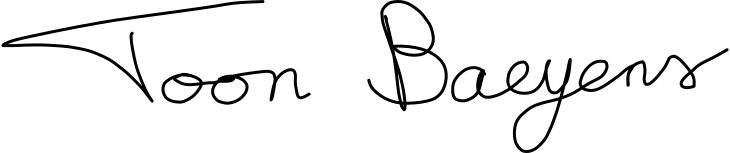
\includegraphics[width=4cm]{img/signature.pdf}\\
    June 2023
\end{flushright}

\stopchapter

